%%%%%%%%%%%%%%%%%%%%%%%%%%%%%%%%%%%%%%%%%
% Structured General Purpose Assignment
% LaTeX Template
%
% This template has been downloaded from:
% http://www.latextemplates.com
%
% Original author:
% Ted Pavlic (http://www.tedpavlic.com)
%
% Note:
% The \lipsum[#] commands throughout this template generate dummy text
% to fill the template out. These commands should all be removed when 
% writing assignment content.
%
%%%%%%%%%%%%%%%%%%%%%%%%%%%%%%%%%%%%%%%%%

\documentclass{article}

\usepackage{fancyhdr} % Required for custom headers
\usepackage{lastpage} % Required to determine the last page for the footer
\usepackage{extramarks} % Required for headers and footers
\usepackage{graphicx} % Required to insert images
\usepackage[latin1]{inputenc}

% Margins
\topmargin=-0.45in
\evensidemargin=0in
\oddsidemargin=0in
\textwidth=6.5in
\textheight=9.0in
\headsep=0.25in 

\linespread{1.1} % Line spacing



\setlength\parindent{0pt} % Removes all indentation from paragraphs

%----------------------------------------------------------------------------------------
%	DOCUMENT STRUCTURE COMMANDS
%	Skip this unless you know what you're doing
%----------------------------------------------------------------------------------------

% Header and footer for when a page split occurs within a problem environment
\newcommand{\enterProblemHeader}[1]{
\nobreak\extramarks{#1}{#1 continued on next page\ldots}\nobreak
\nobreak\extramarks{#1 (continued)}{#1 continued on next page\ldots}\nobreak
}

% Header and footer for when a page split occurs between problem environments
\newcommand{\exitProblemHeader}[1]{
\nobreak\extramarks{#1 (continued)}{#1 continued on next page\ldots}\nobreak
\nobreak\extramarks{#1}{}\nobreak
}

\setcounter{secnumdepth}{0} % Removes default section numbers
\newcounter{homeworkProblemCounter} % Creates a counter to keep track of the number of problems
%----------------------------------------------------------------------------------------
%	NAME AND CLASS SECTION
%----------------------------------------------------------------------------------------

\newcommand{\lessonNumber}[1]{Lezione\ \##1} % Assignment title
\newcommand{\lessonDate}[4]{#1,\ #2\ #3\ #4} % Due date
\newcommand{\lessonCourse}[1]{#1} % Course/class
\newcommand{\lessonTime}[1]{#1} % Class/lecture time
\newcommand{\lessonTeacher}[1]{#1} % Teacher/lecturer
\newcommand{\lessonAuthor}[1]{#1} % Your name

% Set up the header and footer
\pagestyle{fancy}
\lhead{\lessonAuthor{Luca De Franceschi}} % Top left header
\chead{\lessonAuthor{Christian Cardin}\ \lessonTime{9:30}: \lessonNumber{12}} % Top center header
\rhead{\firstxmark} % Top right header
\lfoot{\lastxmark} % Bottom left footer
\cfoot{} % Bottom center footer
\rfoot{Page\ \thepage\ of\ \pageref{LastPage}} % Bottom right footer
\renewcommand\headrulewidth{0.4pt} % Size of the header rule
\renewcommand\footrulewidth{0.4pt} % Size of the footer rule

%----------------------------------------------------------------------------------------
%	TITLE PAGE
%----------------------------------------------------------------------------------------

\title{
\vspace{2in}
\textmd{\textbf{\lessonNumber{12}}\\
\normalsize\vspace{0.1in}\small{\lessonDate{Lunedì}{04}{Novembre}{2013}}\\
\vspace{0.1in}\large{\textit{\lessonTeacher{Christian Cardin},\ \lessonTime{09:30-11:15}}}
\vspace{3in}
}
}

\author{\textbf{\lessonAuthor{Luca De Franceschi}}}
\date{} % Insert date here if you want it to appear below your name

%----------------------------------------------------------------------------------------

\begin{document}

\maketitle
\newpage
\newpage

Caratteristiche varie sui diagrammi delle classi.\\
\textbf{Attributi o operazioni statiche}, non associati ad un oggetto ma al tipo; tutte le istanze la condividono. In UML basta \underline{sottolineare} l'attributo o l'operazione. L'utilizzo di variabili e metodi statici va normalmente evitato, perchè si rischia di tornare alla programmazione procedurale.\\
Inserimento di un sacco di \textbf{parole chiave}, come \texttt{<<interface>>} o \texttt{{abstract\}} o \texttt{<<enumeration>>}. I blocchi di una classe in verità sono più di 3, un blocco per le \textbf{eccezioni} e informazioni aggiuntive sulle responsabilità (commenti). Ma se la classe cambia spesso non ha senso aggiungere queste ultime due, altrimenti avrò problemi in fase di manutenzione. La documentazione deve restare il più possibile allineata con il \textit{codice sorgente}.\\
Si possono inserire delle proprietà derivate nei diagrammi delle classi.

\begin{center}

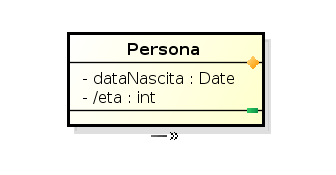
\includegraphics[width=0.75\columnwidth]{img1} % Example image

\end{center}

con la \textit{slash} prima di età dico che età dipende dalla data di nascita. In questo modo evito di scrivere un campo dati in più e quindi scrivo meno codice.\\
Proprietà \textbf{read-only}, non deve fornire i servizi di scrittura su quella classe (niente metodi \textit{setter}); \textbf{frozen} significa che è una costante, l'attributo non può essere modificato.\\
I linguaggi di programmazione forniscono i \textit{template}, classi parametriche. In UML si rappresentano con un rettangolo con bordo tratteggiato in alto a destra della classe. 

\begin{center}

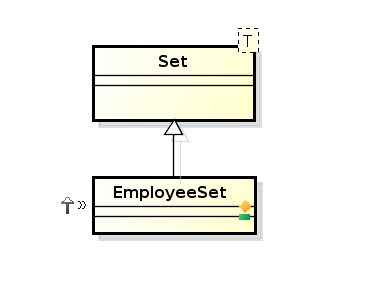
\includegraphics[width=0.75\columnwidth]{img2} % Example image

\end{center}

Le \textbf{classi attive} sono classi che possono essere eseguite (in Java le classi che estendono \textit{Thread}).\\
I diagrammi delle classi sono tra i più ricchi in assoluto, sono stati arricchiti sempre di più, noi ne abbiamo visto solo una parte. Meglio prima partire con diagrammi semplici per prendere confidenza.\\
I \textbf{diagrammi a oggetti} sono molto simili, fotografano il software in un certo istante.\\
\textbf{Esercizio}: cantina formata da più locali, ogni stanza ha scaffali e su questi ci sono diverse bottiglie. Le bottiglie vengono portate da una stanza all'altra ma vogliamo mantenere uno storico di dove è stata quella bottiglia.

\begin{center}

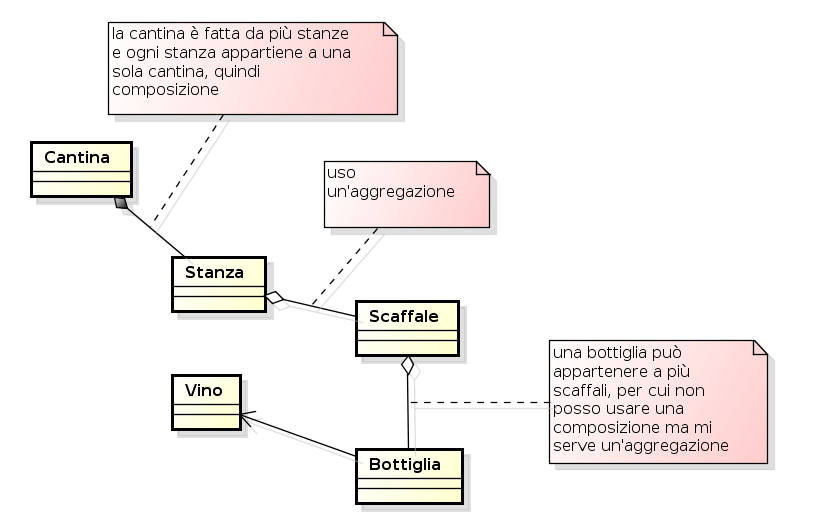
\includegraphics[width=0.75\columnwidth]{img3} % Example image

\end{center}

\textbf{Diagrammi delle attività}\\\\

Finora abbiamo visto il punto dell'analista (\textit{casi d'uso}) e quello del progettista (\textit{classi}). Non abbiamo ancora nessuna tipologia di diagramma che mi permetta di descrivere gli aspetti dinamici del software. Li andremo a scoprire con i \textbf{diagrammi delle attività}. Essi vengono usati sia nella prima parte che nella seconda. Assomiglia molto ad un diagramma di flusso, è una serie di azioni che devono essere effettuate per un processo. Ciascun processo ha un \textbf{nodo iniziale} e un \textbf{nodo finale}.

\begin{center}

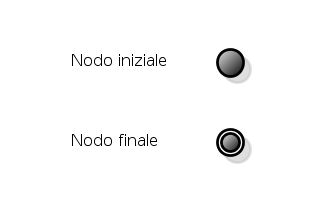
\includegraphics[width=0.75\columnwidth]{img4} % Example image

\end{center}

Da questi due nodi dobbiamo costruire un percorso per andare dallo stato iniziale a quello finale. Questo percorso descrive come l'attività debba essere eseguita. Ogni azione è descritta da un rettangolo con i bordi smussati e ha una descrizione interna. Una decisione, o \textbf{branch}, serve per modellare le condizioni (gli \textit{if}). La condizione si chiama \textbf{guardia}. L'insieme dei rami deve dare la totalità delle condizioni. Quando due o più branch si riuniscono abbiamo un \textbf{merge} che raggruppa il flusso.

\begin{center}

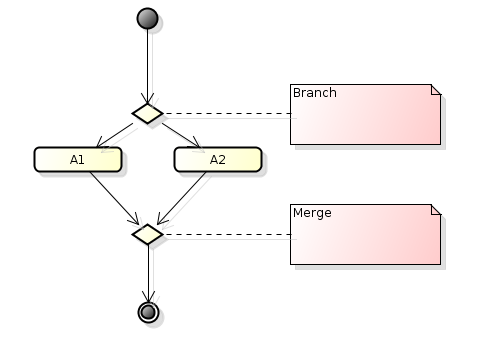
\includegraphics[width=0.75\columnwidth]{img5} % Example image

\end{center}

Questo diagramma mi permette di modellare anche il parallelismo. Questa fase parallela è detta \textbf{fork}. Il fork sdoppia un token in tante azioni che vengono eseguite in parallelo, o in sequenza se non ci interessa l'ordine di esecuzione dei rami. Per ricollegare più flussi paralleli usiamo la \textbf{join}.

\begin{center}

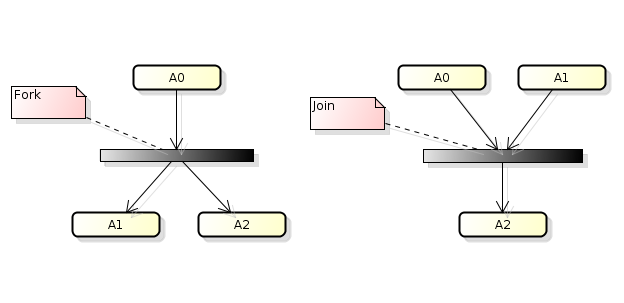
\includegraphics[width=0.75\columnwidth]{img6} % Example image

\end{center}

La join potrebbe avere delle espressioni booleane che consentono di proseguire solo se queste condizioni sono soddisfatte.\\
Può succedere che uno dei flussi, per qualche condizione, \textbf{muoia}, ovvero non abbia delle condizioni di terminazione. In questo caso non termina l'intera attività ma solo quel ramo.\\
Può esserci il caso, soprattutto all'inizio, in cui ho bisogno di definire delle \textbf{sottoattività} che saranno un'implementazione di un'azione (farla vedere al dettaglio). In un diagramma di attività, tra un'azione e un altro passo passano degli oggetti. Un'azione prende un oggetto in input e restituisce un oggetto in output.

\begin{center}

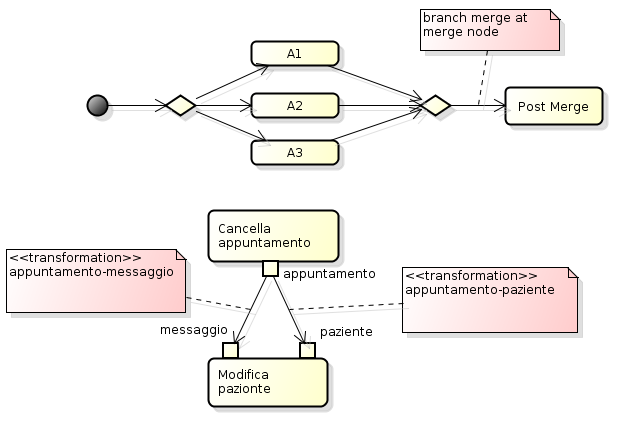
\includegraphics[width=0.75\columnwidth]{img7} % Example image

\end{center}

Le \textbf{partizioni} forniscono una responsabilità all'esecuzione delle azioni.

\end{document}